\documentclass[12pt]{article}

\usepackage{ishn}

\makeindex[intoc]

\begin{document}

\hypersetup{pageanchor=false}
\begin{titlepage}
	\begin{center}
		\vspace*{1em}
		\Huge
		\textbf{III Statistical Field Theory}

		\vspace{1em}
		\large
		Ishan Nath, Michaelmas 2024

		\vspace{1.5em}

		\Large

		Based on Lectures by Prof. Harvey Reall

		\vspace{1em}

		\large
		\today
	\end{center}
	
\end{titlepage}
\hypersetup{pageanchor=true}

\tableofcontents

\newpage

% lecture 1

\setcounter{section}{-1}

\section{Introduction}%
\label{sec:intro}

Office hours: Friday 2-3pm, in B2.09. We are following Tong's notes and example sheets.

Books include the one by Goldenfeld, and Kardar.

\subsection{Motivation}%
\label{sub:motive}

\emph{Universality}: sometimes very different physical systems exhibit the same behaviour, for example a liquid-gas system.

\begin{center}
	
\begin{tikzpicture}[scale=1.2, every node/.style={font=\small}]

    % Axes
    \draw[->] (0,0) -- (8,0) node[below] {Temp $T$};
    \draw[->] (0,0) -- (0,6) node[left] {Pressure $p$};
    
    % Labels for phases
    % \node at (1.5,4) {Solid};
    \node at (5,1.5) {Gas};
    \node at (2.5,5) {Liquid};
    
    % Critical point
    \filldraw (6,3.5) circle (2pt) node[right] {Critical point};
    
    % Coexistence curve
    \draw[thick] (0.8,5) .. controls (2,3.5) and (5,2) .. (6,3.5);
    
    % Triple point
    \filldraw (0.8,5) circle (2pt);
    
    % Dashed line to separate liquid and solid
    \draw[dashed] (0.8,5) -- (0.8,0) node[below] {Melting/Freezing line};
    
    % Saturation line
    \draw[dotted, thick] (6,3.5) -- (6,0) node[below] {Critical Temp};

    % Pressure and Temperature labels (optional customization)
    %\node at (7.8,-0.3) {T};
    %\node at (-0.3,5.8) {P};

\end{tikzpicture}
\end{center}

\begin{center}
\begin{tikzpicture}[scale=1.2, every node/.style={font=\small}]

    % Axes
    \draw[->] (0,0) -- (8,0) node[below] {Density $\rho$};
    \draw[->] (0,0) -- (0,6) node[left] {Temperature $T$};
    
    % Labels for phases
    \node at (6.5,4.5) {Liquid};
    \node at (1.5,4.5) {Gas};
    \node at (4,1) {Coexistence Region};
    
    % Critical point
    \filldraw (4,5) circle (2pt) node[right] {Critical point};
    
    % Coexistence curve (binodal)
    \draw[thick] (1,0.5) .. controls (1.5,2.5) and (2.5,4.5) .. (4,5);
    \draw[thick] (4,5) .. controls (5.5,4.5) and (6.5,2.5) .. (7,0.5);
    
    % Dotted line at critical temperature
    \draw[dotted] (4,5) -- (4,0) node[below] {Critical Density};
    
    % Temperature and Density labels (optional customization)
    %\node at (7.8,-0.3) {$\rho$};
    %\node at (-0.3,5.8) {$T$};

    % Saturation lines (isotherms below critical temperature)
    \draw[dashed] (1.3,3.5) -- (6.7,3.5) node[right] {Isotherms};

\end{tikzpicture}
\end{center}

Experimentally,
\[
|\rho_t - \rho_c| \propto |T - T_c|^\beta,
\]
for $\beta \simeq 0.327$.

Now consider a ferromagnet, where $T_c$ is the Curie temperature. For $T > T_c$, the magnetization is $M = 0$, however for $T < T_c$, $T \sim T_c$, we find
\[
M \propto (T_c - T)^\beta,
\]
where the coefficient $\beta$ is experimentally also $0.327$. We want to know why this is, and also why $\beta$ is this constant.

In this course, we are looking at the classical statistical mechanics of fields.

\newpage

\section{From Spins to Fields}%
\label{sec:spin2field}

\subsection{The Ising Model}%
\label{sub:ising}

This is a simple model for a magnet. In $d$ spatial dimensions, consider a lattice with $N$ sites. On the $i$'th site, we have a `spin' $s_i \in \{-1, 1\}$.

A configuration of spins $\{s_i\}$ has energy
\[
E = - B \sum_i s_i - J \sum_{\langle i, j\rangle} s_i s_j.
\]
An important question is, how does the physics depend on the parameters $B, J$ and $T$?

If $J > 0$, then the spins prefer to align, as $\uparrow \uparrow$ or $\downarrow \downarrow$. This is a ferromagnet. If $J < 0$, the spins prefer to antialign, as $\uparrow \downarrow$ or $\downarrow \uparrow$. This is an antiferromagnet.

Assume that $J > 0$. If $B > 0$, then the spins prefer to be $\uparrow$, and for $B < 0$, the spins prefer to be $\downarrow$.

Now let's consider changing temperature. Intuitively, for low temperature $T$, the system prefers to minimize $E$, which gives an ordered state. For high $T$, we want to maximize $S$, the entropy, which gives a disordered state.

In the canonical ensemble, we have
\[
	p[s_i] = \frac{e^{-\beta E[s_i]}}{Z},
\]
where we recall $\beta = 1/T$. Moreover we always assume $k_B = 1$. Here $Z$ is the partition function
\[
	Z(T, B) = \sum_{\{s_i\}} e^{-\beta E[s_i]}.
\]
The \emph{thermodynamic free energy}\index{thermodynamic free energy} is
\[
F_{\mathrm{thermo}}(T, B) = \langle E \rangle - TS = - T \log Z.
\]
Another observable is the \emph{magnetization}\index{magnetization}
\[
	m = \frac{1}{N} \left\langle \sum_{i = 1}^n s_i \right \rangle \in [-1, 1].
\]
This distinguishes ordered phases, where $m \neq 0$, and disordered phases, where $m = 0$. Using the partition function,
\[
	m = \sum_{\{s_i\}} \frac{e^{-\beta[s_i]}}{Z} \cdot \frac{1}{N} \sum_i s_i = \frac{1}{N \beta} \frac{\partial}{\partial B} \log Z.
\]
Therefore it suffices to find the partition function. For $d = 1$, this is easy. For $d = 2$ there is no analytic solution except for the square lattice with $B = 0$.

For the other cases there is no exact solution. Our aim is to approximate in a way that correctly captures long-distance behaviour. We define $m$ for any $\{s_i\}$ by
\[
m = \frac{1}{N} \sum s_i.
\]
Then write
\[
	Z = \sum_m \sum_{\{s_i\} \mid m} e^{-\beta E[s_i]} := \sum_m e^{-\beta F(m)}.
\]
Notice changing $s_i$ changes $m$ by $2/N$ so $m$ is quantized into distances of $2/N$. For large $N$, we can approximate this as continuous, so
\[
	Z \approx \frac{N}{2} \int_{-1}^1 \diff m \, e^{-\beta F(m)}.
\]
$F(m)$ is the \emph{effective free energy}\index{effective free energy}. This depends on $T, B$ and $m$. It contains more information than $F_{\mathrm{thermo}}$. If $f(m) = F(m)/N$, then
\[
Z \propto \int_{-1}^1 \diff m \, e^{-\beta N f(m)}.
\]
For $N$ large, $\beta f(m) = \mathcal{O}(1)$, as it is intensive, so this integral will be dominated by the minimum of $f$, where
\[
\frac{\partial f}{\partial m} \biggr|_{m = m_{\mathrm{min}}} = 0.
\]
Here $m_{\mathrm{min}}$ is the equilibrium value of the magnetization. By the saddle-point approximation,
\[
Z \propto e^{-\beta N f(m_{\mathrm{min}})} = e^{-\beta F(m_{\mathrm{min}})}.
\]
Thus,
\[
F_{\mathrm{thermo}}(T, B) = F(m_{\mathrm{min}}(T, B), T, B).
\]
However computing $F(m)$ is hard. For a first attempt, we use the ``mean field approximation''. Here we replace $s_i$ with $m$, so
\[
E = - B \sum_i m - J \sum_{\langle i, j \rangle} m^2 = - B N m - \frac{1}{2}N J q m^2.
\]
In this, $q$ is the number of nearest neighbours. For $d = 1$, $q = 2$. In general it is $2d$. In this approximation,
\[
	Z \approx \sum_m \Omega(m) e^{-\beta E[m]},
\]
where $\Omega(m)$ is the number of configurations with average value $m$.

% lecture 2

Let $N_\uparrow$ be the number of up spins, and $N_\downarrow = N - N_\uparrow$ the number of down spins. Then,
\[
m = \frac{N_\uparrow - N_\downarrow}{N} = \frac{2N_\uparrow - N}{N},
\]
so
\[
\Omega(m) = \frac{N!}{N_\uparrow!(N - N_\uparrow)!} = \frac{N!}{N_\uparrow! N_\downarrow!}.
\]
By Stirling's approximation,
\[
\log n! = n \log n - n
\]
for large $n$, so
\[
\log \Omega \approx N \log N - N_\uparrow \log N_\uparrow - N_\downarrow \log N_\downarrow.
\]
Dividing by $N$ and substituting in $m$ for $N_\uparrow, N_\downarrow$,
\[
\frac{\log \Omega}{N} \approx \log 2 - \frac{1}{2} (1 + m) \log(1 + m) - \frac{1}{2} (1 - m) \log(1 - m).
\]
Since
\[
e^{-\beta N f(m)} = \Omega(m) e^{-\beta E(m)}
\]
in the mean field approximation, taking the logarithm we find
\[
	f(m) = - B m - \frac{1}{2} J q m^2 - T \left[ \log 2 - \frac{1}{2}(1 + m) \log(1 + m) - \frac{1}{2} (1 - m) \log(1 - m) \right].
\]
We minimize
\begin{align*}
	\frac{\partial f}{\partial m} = 0 &\implies \beta(B + J qm) = \frac{1}{2} \log \left( \frac{1 + m}{1 - m} \right) \\
					  &\implies m = \tanh[\beta(B + Jqm)],
\end{align*}
where $B_{\mathrm{eff}} = B + Jqm$. The intuition is that each spin feels an effective magnetic field, given by the actual magnetic field, and the overall spin.

\subsection{Landau Theory of Phase Transitions}%
\label{sub:pt}

At a phase transition, some quantity (an \emph{order parameter}\index{order parameter}) is not smooth. For us, this is $m$. For small $m$,
\[
f(m) \approx -T \log 2 - B m + \frac{1}{2} (T - Jq)m^2 + \frac{1}{12} Tm^4 + \cdots.
\]
In equilibrium, $m = m_{\mathrm{min}}$: how does this behave as we vary $T$ and $B$?

First we look at $B = 0$. Note the first part does not change the minimization, so
\[
f(m) \approx \frac{1}{2} (T - T_c)m^2 + \frac{1}{12} Tm^4 + \cdots,
\]
where $T_c = Jq$.

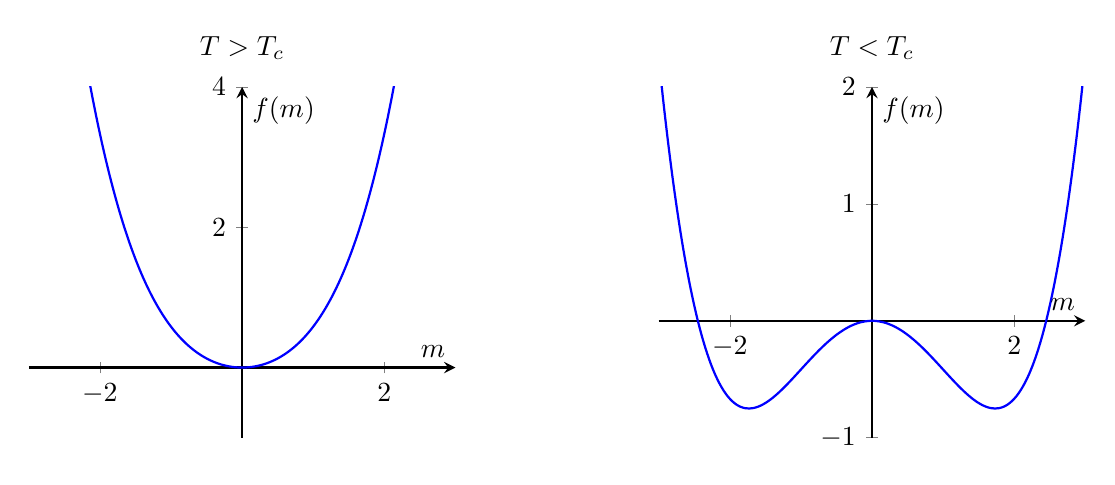
\begin{tikzpicture}

% First plot: T > T_c
\begin{axis}[
    width=7cm,
    title={$T > T_c$},
    axis lines = middle,
    xlabel = {$m$},
    ylabel = {$f(m)$},
    samples=100,
    domain=-3:3,
    xmin=-3, xmax=3,
    ymin=-1, ymax=4,
    smooth,
    thick
]
% Free energy function for T > T_c
\addplot[
    blue,
    thick,
] {0.5*(1)*x^2 + (1/12)*x^4}; % f(m) = 1/2(T-T_c)m^2 + 1/12Tm^4 for T > T_c
\end{axis}

% Second plot: T < T_c (next to the first)
\begin{axis}[
    width=7cm,
    xshift=8cm, % Shift second plot horizontally
    title={$T < T_c$},
    axis lines = middle,
    xlabel = {$m$},
    ylabel = {$f(m)$},
    samples=100,
    domain=-3:3,
    xmin=-3, xmax=3,
    ymin=-1, ymax=2,
    smooth,
    thick
]
% Free energy function for T < T_c
\addplot[
    blue,
    thick,
] {0.5*(-1)*x^2 + (1/12)*x^4}; % f(m) = 1/2(T-T_c)m^2 + 1/12Tm^4 for T < T_c
\end{axis}

\end{tikzpicture}

For $T < T_c$, $m_{\mathrm{min}} = 0$. For $ < T_c$, $m_{\mathrm{min}} = \pm m_0$, where
\[
	m_0 = \sqrt{\frac{3 (T_c - T)}{T}}.
\]
Hence here is a phase transition at $T = T_c$. For $T > T_c$, we have $m =  0$, which is a disordered phase, and for $T < T_c$, $m \neq 0$, giving an ordered phase.


\begin{center}
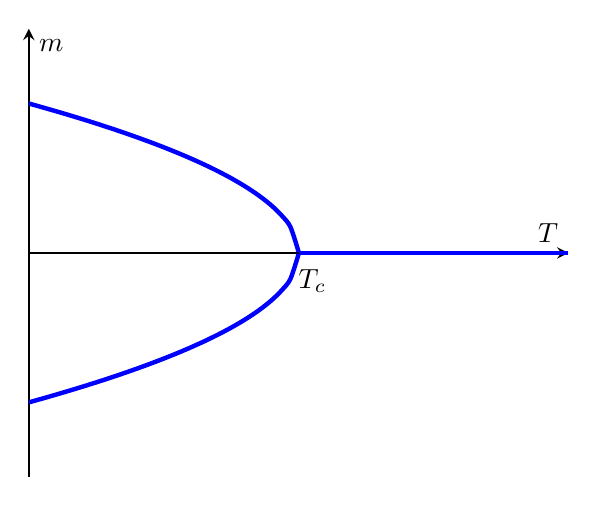
\begin{tikzpicture}

\begin{axis}[
    axis lines = middle,
    xlabel = {$T$},
    ylabel = {$m$},
    samples=100,
    domain=-1:2,
    xmin=0, xmax=2,
    ymin=-1.5, ymax=1.5,
    xtick={1},
    xticklabels={$T_c$},
    xticklabel style = {xshift=5pt},
    ytick={0},
    smooth,
    thick
]

% Plot the bifurcation diagram
\addplot[
    blue,
    ultra thick,
] {-sqrt(1-x)};  % Lower branch for T < T_c (m < 0)
\addplot[
    blue,
    ultra thick,
] {sqrt(1-x)};   % Upper branch for T < T_c (m > 0)
\addplot[
    blue,
    ultra thick,
    domain=1:2
] {0};           % m = 0 for T >= T_c

\end{axis}
\end{tikzpicture}
\end{center}

Here, $m$ is continuous at $T = T_c$, giving a continuous phase transition, or second order phase transition.

Note that $F$ is invariant under $\mathbb{Z}_2$ symmetry: if we swap $m \to -m$, and $B \to -B$. For $T < T_c$, either $m = +m_0$ or $m = -m_0$, the $\mathbb{Z}_2$ symmetry does not preserve the ground state, known as `spontaneous symmetry breaking' (SSB).

At finite $N$, $Z$ is \emph{analytic} in $T, B$. Therefore the phase transition only occurs for $N \to \infty$, and SSB also only occurs for $N \to \infty$: in this case
\[
m = \lim_{B \to 0} \lim_{N \to \infty} \frac{1}{N} \sum \langle s_i \rangle.
\]
Note the order of the limits are important, otherwise we get 0.

For finite $N$, the $\mathbb{Z}_2$ symmetry tells us $F_{\mathrm{thermo}}$ is even in $B$, so
\[
	\langle m \rangle = - \frac{1}{N} \frac{\partial F_{\mathrm{thermo}}}{\partial B} \biggr|_{B= 0} = 0.
\]
The heat capacity is
\[
C = \frac{\partial \langle E \rangle}{\partial T}, \qquad \braket E = - \frac{\partial \log Z}{\partial \beta}.
\]
Thus we find
\[
C = \beta^2 \frac{\partial^2 \log Z}{\partial \beta^2},
\]
and notice that
\[
\log Z = - \beta N f(m_{\mathrm{min}}) = 
\begin{cases}
	\text{const} & T > T_c, \\
	\frac{3N}{4} \frac{(T_c - T)^2}{T^2} + \text{const} & T< T_c,
\end{cases}
\]
so
\[
c = \frac{C}{N} \to
\begin{cases}
	0 & T \to T_c^+, \\
	3/2 & T \to T_c^-.
\end{cases}
\]
Therefore $c$ is discontinuous at $T = T_c$.

For $B > 0$, we find
\[
f(m) = -Bm + \frac{1}{2}(T - T_c)m^2 + \frac{1}{12} Tm^4 + \cdots
\]

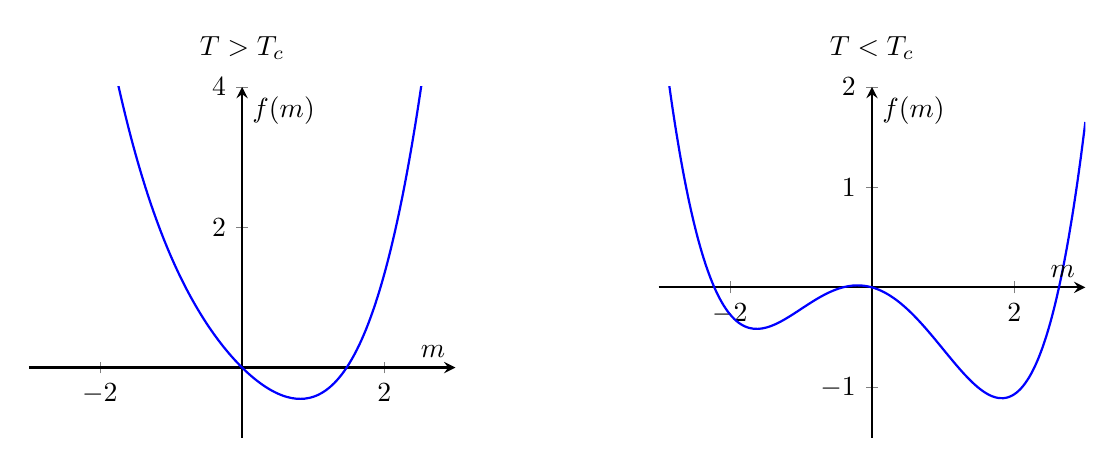
\begin{tikzpicture}

% First plot: T > T_c
\begin{axis}[
    width=7cm,
    title={$T > T_c$},
    axis lines = middle,
    xlabel = {$m$},
    ylabel = {$f(m)$},
    samples=100,
    domain=-3:3,
    xmin=-3, xmax=3,
    ymin=-1, ymax=4,
    smooth,
    thick
]
% Free energy function for T > T_c
\addplot[
    blue,
    thick,
] {-x + 0.5*(1)*x^2 + (1/12)*x^4}; % f(m) = 1/2(T-T_c)m^2 + 1/12Tm^4 for T > T_c
\end{axis}

% Second plot: T < T_c (next to the first)
\begin{axis}[
    width=7cm,
    xshift=8cm, % Shift second plot horizontally
    title={$T < T_c$},
    axis lines = middle,
    xlabel = {$m$},
    ylabel = {$f(m)$},
    samples=100,
    domain=-3:3,
    xmin=-3, xmax=3,
    ymin=-1.5, ymax=2,
    smooth,
    thick
]
% Free energy function for T < T_c
\addplot[
    blue,
    thick,
] {-0.2*x + 0.5*(-1)*x^2 + (1/12)*x^4}; % f(m) = 1/2(T-T_c)m^2 + 1/12Tm^4 for T < T_c
\end{axis}
\end{tikzpicture}

In this case,
\[
m_{\mathrm{min}} = \frac{B}{T},
\]
for $T \to \infty$.

In this case $m_{\mathrm{min}}$ depends smoothly on $T$, so there is no phase transition if $T$ is varied at fixed $B \neq 0$.

\begin{center}
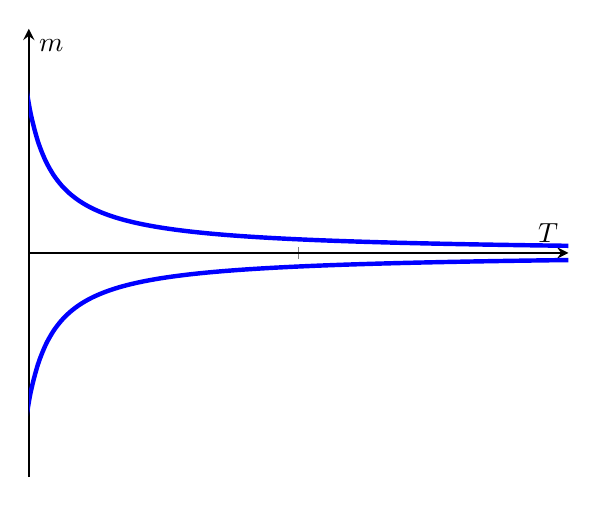
\begin{tikzpicture}

\begin{axis}[
    axis lines = middle,
    xlabel = {$T$},
    ylabel = {$m$},
    samples=100,
    domain=-1:2,
    xmin=0, xmax=2,
    ymin=-1.5, ymax=1.5,
    xtick={1},
    xticklabels={},
    ytick={0},
    smooth,
    thick
]

% Plot the bifurcation diagram
\addplot[
    blue,
    ultra thick,
] {1 / (1 + 10 * x)};  % Lower branch for T < T_c (m < 0)
\addplot[
    blue,
    ultra thick,
] {-1 / (1 + 10 * x)};   % Upper branch for T < T_c (m > 0)

\end{axis}
\end{tikzpicture}
\end{center}

But, if we vary $B$ at fixed $T < T_c$, then $m$ jumps discontinuously from $m_0$ to $-m_0$ as $B$ decreases from positive to negative, which is an example of a first order phase transition.

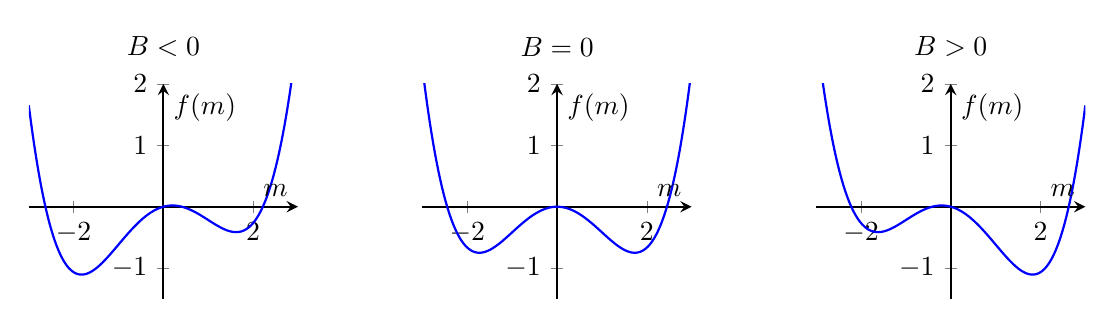
\begin{tikzpicture}

\begin{axis}[
    width=5cm,
    xshift=-5cm,
    title={$B < 0$},
    axis lines = middle,
    xlabel = {$m$},
    ylabel = {$f(m)$},
    samples=100,
    domain=-3:3,
    xmin=-3, xmax=3,
    ymin=-1.5, ymax=2,
    smooth,
    thick
]
% Free energy function for T > T_c
\addplot[
    blue,
    thick,
] {0.2 * x + 0.5*(-1)*x^2 + (1/12)*x^4}; % f(m) = 1/2(T-T_c)m^2 + 1/12Tm^4 for T > T_c
\end{axis}

\begin{axis}[
    width=5cm,
    title={$B = 0$},
    axis lines = middle,
    xlabel = {$m$},
    ylabel = {$f(m)$},
    samples=100,
    domain=-3:3,
    xmin=-3, xmax=3,
    ymin=-1.5, ymax=2,
    smooth,
    thick,
]
% Free energy function for T > T_c
\addplot[
    blue,
    thick,
] {0.5*(-1)*x^2 + (1/12)*x^4}; % f(m) = 1/2(T-T_c)m^2 + 1/12Tm^4 for T > T_c
\end{axis}

% Second plot: T < T_c (next to the first)
\begin{axis}[
    width=5cm,
    xshift=5cm, % Shift second plot horizontally
    title={$B > 0$},
    axis lines = middle,
    xlabel = {$m$},
    ylabel = {$f(m)$},
    samples=100,
    domain=-3:3,
    xmin=-3, xmax=3,
    ymin=-1.5, ymax=2,
    smooth,
    thick
]
% Free energy function for T < T_c
\addplot[
    blue,
    thick,
] {-0.2*x + 0.5*(-1)*x^2 + (1/12)*x^4}; % f(m) = 1/2(T-T_c)m^2 + 1/12Tm^4 for T < T_c
\end{axis}
\end{tikzpicture}


\begin{center}
\begin{tikzpicture}
\begin{axis}[
    axis lines = middle,
    xlabel = {$T$},
    ylabel = {$B$},
    xmin=0, xmax=2,
    ymin=-1.5, ymax=1.5,
    xtick={1},
    xticklabels={$T_c$},
    ytick={0},
    samples=100,
    smooth,
    thick
]

% Plot the critical isothermal line at T = T_c
\addplot[
    domain=0:1,
    ultra thick,
    red
] (x,0);  % Critical isothermal line at T = T_c


% Critical point at (T_c, 0)
\node[red, fill=red, circle, inner sep=2pt] at (axis cs:1,0) {};

\end{axis}
\end{tikzpicture}
\end{center}

We can draw the phase transition points as above.

% lecture 3

Consider the behaviour near the critical point. If we fix $T = T_c$, then
\[
f \approx - B m + \frac{1}{12} Tm^4 + \cdots,
\]
so minimizing, we see that $m^3 \sim B$, and $m \sim B^{1/3}$.

We can also define the \emph{magnetic susceptibility}\index{magnetic susceptibility} as
\[
\chi = \left( \frac{\partial m}{\partial B} \right)_T.
\]
For $T > T_c$,
\[
f(m) = - Bm + \frac{1}{2} (T - T_c)m^2 + \cdots,
\]
so
\[
m \approx \frac{B}{T - T_c} \implies \chi = \frac{1}{T - T_c}.
\]
For $T < T_c$, we write $m = m_0 + \delta m$, and solving for $\delta m$ to leading order, we find
\[
m = m_0 + \frac{B}{2(T_c - T)} \implies \chi = \frac{1}{2(T_c - T)}.
\]
Hence,
\[
\chi \sim \frac{1}{|T-T_c|}.
\]

We have been using the MFT approximation. Does this give the correct results?
\begin{itemize}
	\item $d=1$. No, there is no phase transition.
	\item $d = 2, 3$. The phase diagram is qualitatively correct, but the qualitative predictions at the critical point are incorrect.
	\item $d \geq 4$. Yes.
\end{itemize}

Similarly for other systems, MFT gets the phase structure wrong for $d \leq d_l$, the `lower critical dimension', and correct for $d \geq d_c$, the `upper critical dimension'. In the Ising model, $d_l = 1$ and $d_c = 4$.

For $d_l < d < d_c$, the theory is interesting.

\subsection{Critical Exponents}%
\label{sub:ce}

Near the critical point, MFT predicts the following:
\begin{itemize}
	\item If $B = 0$, then as $T \to T_c^{-}$,
		\begin{align*}
			m &\sim (T_c - T)^\beta & \text{with } &\beta = \frac{1}{2}, \\
			c &\sim c_{\pm} |T - T_c|^{-\alpha} & \text{with } &\alpha = 0, \\
			\chi &\sim \frac{1}{|T - T_c|^\gamma} & \text{with } &\gamma = 1.
		\end{align*}
	\item As $B \to 0$,
		\[
			m \sim B^{1/\delta} \qquad \text{with } \delta = 3.
		\]
\end{itemize}

Here, $\alpha, \beta, \gamma, \delta$ are the \emph{critical exponents}\index{critical exponents}.

These values are not correct for small $d$.

\begin{table}[ht]
\centering
\begin{tabular}{c|ccc}
	& MFT & $d = 2$ & $d = 3$ \\
\hline
	$\alpha$ & $0$ (disc) & $0$ (log) & 0.1101.. \\
	$\beta$ & $\frac{1}{2}$ & $\frac{1}{8}$ & 0.3264.. \\
	$\gamma$ & $1$ & $\frac{7}{4}$ & 1.2371..\\
	$\delta$ & $3$ & $15$ & 4.7898..
\end{tabular}
\caption{Predictions and Theoretical Critical Exponents}
\end{table}

\subsection{Universality}%
\label{sub:univ}

\begin{center}
\begin{tikzpicture}
\begin{axis}[
    width=10cm,
    %title={$B = 0$},
    axis lines = middle,
    xlabel = {$T$},
    ylabel = {$p$},
    samples=100,
    domain=0:4,
    xmin=0, xmax=4,
    ymin=0, ymax=1.5,
    xtick = {0},
    ytick = {0},
    smooth,
    thick
]
% Free energy function for T > T_c
\addplot[
    blue,
    thick,
    ] {x^3 * 0.1 - x^4 * 0.02};

\addplot[
    blue,
    thick,
    domain = 2:3.5
    ] {x * 0.24};

\node[red, fill=blue, circle, inner sep=2pt] at (axis cs:3.5,3.5*0.24) {};

\node at (axis cs:1,0.75) {Solid};
\node at (axis cs:3,0.86) {Liquid};
\node at (axis cs:3,0.5) {Gas};

\end{axis}
\end{tikzpicture}
\end{center}

In a normal material, we have liquid-gas phase transition similar to the Ising model; a line of first order phase transitions, ending at a critical point.

If we replace $B$ with $p$ the pressure, and $m$ with $v = V/N$ as our orde parameter, then using an equation of state (e.g. the van der Waals) to calculate the behaviour near the critical point:
\begin{itemize}
	\item As $T \to T_c$,
		\[
			v_{\mathrm{gas}} - v_{\mathrm{liquid}} \sim (T_c - T)^\beta \qquad \text{where } \beta = \frac{1}{2}.
		\]
	\item If $T = T_c$ is fixed, and $p \to p_c$,
		\[
			v_{\mathrm{gas}} - v_{\mathrm{liquid}} \sim (p - p_c)^{1/\delta} \qquad \text{where } \delta = 3.
		\]
	\item The isothermal compatibility is
		\[
			\kappa = - \frac{1}{v} \left( \frac{\partial v}{\partial p} \right)_T \sim \frac{1}{|T - T_c|\gamma} \qquad \text{where } \gamma = 1.
		\]
	\item The heat capacity is
		\[
			c_v \sim c_{\pm} |T - T_c|^{-\alpha} \qquad \text{where }\alpha = 0,
		\]
		i.e. the heat capacity is discontinuous.
\end{itemize}

These are the same predictions as for MFT for the Ising model. As is probably is expected, these are incorrect; but the correct values are the same as the correct values for $d = 3$ Ising model!

This is an example of \emph{universality}\index{universality}: different physical systems can exhibit the same behaviour at the critical points.

This suggests that the microscopic physics is unimportant at a critical point. Systems governed by the same critical point belong to the same \emph{universality class}\index{universality class}.

\subsection{Landau-Ginzberg Theory}%
\label{sub:lgt}

Our aim is to find a model that correctly describes long-distance physics near the critical point, which can be used to calculate critical exponents for all theories in the same universality class.

LG theory generalizes MFT, to allow for spatial variation in $m$.

Here, $m(\mathbf{x})$ is a field, produced from a microscopic model by coarse-graining. In the Ising model, we divide the lattice into boxes, each with $N' \ll N$ sites, with size $a$. Then we can define
\[
	m(\mathbf{x}) = \text{average of spins in box with centre } \mathbf{x}.
\]
Take $N' \gg 1$ the discreteness of $m(\mathbf{x})$ can be ignored, and $m \in [-1, 1]$.

Assume that $a \ll \xi$, the length scale over which the physics varies. Treat $m(\mathbf{x})$ as a smooth function, which does not vary on scales less than $a$. Then,
\[
	Z = \sum_{m(\mathbf{x})} \sum_{\{s_i\} | m(\mathbf{x})} e^{-\beta E[s_i]} = \sum_{m (\mathbf{x})} e^{-\beta F[m(\mathbf{x})]}.
\]
Here, $F[m(\mathbf{x})]$ is a \emph{functional}, which depends on a functional. This is the \emph{Landau-Ginzberg free energy}\index{Landau-Ginzberg free energy}.

We write
\[
	Z = \int \mathcal{D} m(\mathbf{x}) \, e^{-\beta F[m(\mathbf{x})]},
\]
which is a \emph{functional integral}\index{functional integral}, a sum over all $m(\mathbf{x})$ that do not vary on scales less than $a$.

% lecture 4

We can interpret this as a probability of a field configuration $m(\mathbf{x})$ as
\[
	p[m(\mathbf{x})] = \frac{e^{-\beta F[m(\mathbf{x})]}}{Z}.
\]
The form of $F[m(\mathbf{x})]$ is constrained by the following:
\begin{itemize}
	\item Locality: spins only influence nearby spins, so we may write
		\[
			F[m(\mathbf{x})] = \int \Diff dx\, f(m(\mathbf{x}), \nabla_i m(\mathbf{x}), \nabla_i \nabla_j m(\mathbf{x}), \ldots),
		\]
		not for example a function in $x$ and $y$.
	\item Translational symmetry is inherited from discrete translational symmetry of the lattice.
	\item Can also inherit rotational symmetry.
	\item We also have a $\mathbb{Z}_2$ symmetry, by $s_i \to -s_i$, and $B \to -B$. So we can assume that $F$ is invariant under $m(\mathbf{x}) \to - m(\mathbf{x})$, and $B \to -B$.
	\item Analyticity. We assume $F[m(\mathbf{x})]$ is defined by coarse graining over a finite number of spins. This lets us suppose $f$ is \emph{analytic}, i.e. we can Taylor expand near $m = 0$.
\end{itemize}

From dimensional analysis,
\[
a \nabla m \sim \frac{a m}{\xi}, \qquad a^2 \nabla \nabla m \sim \frac{a^2 m}{\xi^2}.
\]
The fact $\xi \gg a$ suggests that $\nabla m$ is more important than $\nabla \nabla m$, etc.

From the above assumptions, for $B = 0$ we can write
\[
	F[m(\mathbf{x})] = \int \Diff4 x \left( \frac{1}{2} \alpha_2(T) m^2 + \frac{1}{4} \alpha^4 m^4 + \frac{1}{2} \gamma(T) (\nabla m)^2 + \cdots \right).
\]
If $B \neq 0$, we could include $Bm, Bm^3$ terms.

The coefficients $\alpha_2(T), \alpha_4(T)$ are hard to compute from first principles. From MFT, we expect that $\alpha_2(T) \sim T - T_c$, and $\alpha_4(T) \sim T/3$. But all we will assume is that the coefficients are analytic in $T$, with $\alpha_4(T) > 0$, $\gamma(T) > 0$, and $\alpha_2(T) > 0$ for $T > T_c$, with a simple zero at $T = T_c$.

Still, this field integral is hard to evaluate. Hence we will use a saddle point approximation.

Assume that the integral is dominated by the saddle point; the $m(\mathbf{x})$ that minimizes $F[m(\mathbf{x})]$. We can vary $m(\mathbf{x}) \to m(\mathbf{x}) + \delta m(\mathbf{x})$, with
\begin{align*}
\delta F &= \int \Diff 4 x (\alpha_2 m \delta m + \alpha_4 m^3 \delta m + \gamma \nabla m \cdot \nu \delta m + \cdots ) \\
		   &= \int \Diff 4 x (\alpha_2 m + \alpha_4 m^3 - \gamma \nabla ^2 m + \cdots ) \delta m,
\end{align*}
by using integration by parts. The part in the brackets is often written as
\[
\frac{\delta F}{\delta m(\mathbf{x})},
\]
the \emph{functional derivative}\index{functional derivative}. If $m(\mathbf{x})$ minimizes $F$, then $\delta F = 0$ for all $\delta m(\mathbf{x})$, so
\[
\gamma \nabla^2 m = \alpha_1 m + \alpha_4 m^3 + \cdots.
\]
This is just the Euler-Lagrange equaions, I think? The simplest solution is when $m$ is constant, which corresponds to MFT/Landau theory.

For $T > T_c$, $\alpha_2 > 0$, so $m = 0$, and for $T < T_c$, $\alpha_2 < 0$, so
\[
	m = \pm m_0 \sqrt{\frac{-\alpha_2}{\alpha_4}}.
\]

\subsection{Domain Walls}%
\label{sub:dw}

If $T < T_c$, then there are two ground states $m = \pm m_0$. We could have $m \to \pm m_0$ as $x \to \pm \infty$.

Consider a field that varies only in $x$, so $m(\mathbf{x}) = m(x)$. Then we need to solve
\[
\gamma \frac{\diff^2 m}{\diff x^2} = \alpha_2 m + \alpha_4 m^3 + \cdots.
\]
This is solved by
\[
m = m_0 \tanh \left( \frac{x - X}{W} \right),
\]
where $X$ is some constant, and $W = \sqrt{-2 \gamma/\alpha_2}$.

\begin{center}
\begin{tikzpicture}
\begin{axis}[
    width=10cm,
    %title={$B = 0$},
    axis lines = middle,
    xlabel = {$x$},
    ylabel = {$m$},
    samples=100,
    domain=-2:2,
    xmin=-2, xmax=2,
    ymin=-1, ymax=1,
    xtick = {0},
    ytick = {0},
    smooth,
    thick
]
% Free energy function for T > T_c
\addplot[
    blue,
    thick,
    ] {tanh((x-0.5)* 0.8)};


%\node at (axis cs:1,0.75) {Solid};

\end{axis}
\end{tikzpicture}
\end{center}

This is a \emph{domain wall}\index{domain wall} with position $X$ and width $W$.

If the system has size $L$, then the free energy is $F[m_0] \propto L^d$. The cost of the domain wall is
\[
	\Delta F = F[m(\mathbf{x})] - F[m_0] \sim L^{d-1} \sqrt{\frac{- \gamma \alpha_2^3}{\alpha_4^2}},
\]
which is proportional to the area of the domain wall.

Near the critical point $\alpha_2 \to 0$ and $W \to \infty$, so $\Delta F \to 0$.

Domain walls explain why $d_l = 1$ for the Ising model. Let $d= 1$, and $-L/2 < x < L/2$, and assume $\alpha_2(T) < 0$.

The boundary conditions are $m(\pm L/2) = m_0$, and the probability of the configuration is
\[
	\frac{e^{-\beta F[m(\mathbf{x})]}}{Z}.
\]

\begin{center}
\begin{tikzpicture}
\begin{axis}[
    width=10cm,
    %title={$B = 0$},
    axis lines = middle,
    xlabel = {$x$},
    ylabel = {$m$},
    samples=100,
    domain=-2:2,
    xmin=-2, xmax=2,
    ymin=-1, ymax=1,
    xtick = {0},
    ytick = {0},
    smooth,
    thick
]
% Free energy function for T > T_c
\addplot[
    blue,
    thick,
    ] {tanh((x-1)*2)^2 - 2.5 + tanh((x+1)*2)^2 + tanh((x)*2)^2};


%\node at (axis cs:1,0.75) {Solid};

\end{axis}
\end{tikzpicture}
\end{center}

Now consider a field with two domain walls. Assume $L \gg W$. For well separated wells, $\Delta F_{\mathrm{2 wells}} = 2 \Delta F$. Then,
\[
	\frac{\mathbb{P}(2 \text{ domain walls at given } X, Y)}{p(m = m_0)} = e^{-2 \beta \Delta F}.
\]
Summing over all $X, Y$,
\[
	\frac{\mathbb{P}(\text{2 domain walls})}{\mathbb{P}(m = m_0)} \sim \int_{-L/2}^{L/2} \frac{\diff X}{W} \int_{X}^{L/2} \frac{\diff Y}{W} e^{-2 \beta \Delta(F)} \sim \left( \frac{L}{W} \right)^2 e^{-2 \beta \Delta(F)}.
\]
For $d = 1$, the RHS goes to $0$ as $L \to \infty$, showing that energy beats entropy. But for $d = 1$, the RHS tends to $\infty$, as entropy beats energy.

Hence for $d = 1$, it is much more probably to see two domain walls than a constant field, so any region with constant $m = \pm m_0$ is unstable to the formation of domain walls, so the ordered phase does not exist.

% lecture 5

\newpage

\section{My First Path Integral}%
\label{sec:mlp}

We want to go beyond the saddle point approximation to calculate
\[
	Z = \int \mathcal{D} m(\mathbf{x}) \, e^{-\beta F[m(\mathbf{x})]}.
\]
We make a couple of changes: first we change from $m(\mathbf{x})$ to $\phi(\mathbf{x})$, and also we assume $B = 0$, so
\[
	F[\phi(\mathbf{x})] = \int \Diff dx \left( \frac{1}{2} \alpha_2(T) \phi^2 + \frac{1}{4} \alpha_4 \phi^4 + \frac{1}{2}\gamma(T) (\nabla \phi)^2 + \cdots \right).
\]
Evaluating the path integral is:
\begin{itemize}
	\item Easy if $F$ is quadratic in $\phi$.
	\item Possibly if the higher order terms are small.
	\item Very hard otherwise.
\end{itemize}

For $T > T_c$, let $\mu^2 = \alpha_2(T) > 0$. Consider the quadratic approximation to $F$:
\[
	F[\phi(\mathbf{x})] = \frac{1}{2} \int \Diff dx (\mu^2 \phi^2 + \gamma (\nabla \phi)^2).
\]
For $T < T_c$, $\alpha_2(T) < 0$, so $\braket \phi = \pm m_0$. Let $\tilde \phi = \phi - \braket \phi$. Then,
\[
	F = F[m_0] + \frac{1}{2} \int \Diff dx (\alpha_2(T) \tilde \phi^2 + \gamma(T) (\nabla \tilde \phi)^2 + \cdots).
\]
Here
\[
\alpha_2'(T) = \alpha_2(T) + 3 m_0^2 \alpha_4(T) = -2 \alpha_2(T) > 0.
\]
This quadratic approximation gives the same equation with $\phi$ replaced with $\tilde \phi$, and $\mu^2 = \alpha_2'(T) = 2|\alpha_2(T)| > 0$.

\subsection{Thermodynamic Free Energy}%
\label{sub:tfe}

We aim to compute the corrections to $F_{\mathrm{thermo}}$ from the fluctuation in $\phi(\mathbf{x})$. It is useful to take the Fourier transform
\[
\phi_{\mathbf{k}} = \int \Diff d x \, e^{-i \mathbf{k} \cdot \mathbf{x}} \phi(\mathbf{x}),
\]
where since $\phi$ is real, $\phi^\ast_{\mathbf{k}} = \phi_{-{\mathbf{k}}}$. Here the wavevector $\mathbf{k}$ is often called the \emph{momentum}\index{momentum}. Since $\phi$ doesn't vary on scales less than $a$, we get $\phi_{\mathbf{k}} = 0$ for all $|\mathbf{k}| = \Lambda$, where $\Lambda = \pi/a$ is called the ultraviolet cutoff.

The inverse Fourier transform is given by
\[
\phi(\mathbf{x}) = \int \frac{\Diff d x}{(2 \pi)^d} e^{i \mathbf{k} \cdot \mathbf{x}} \phi_{\mathbf{k}}.
\]
In finite volume, consider a system occupying a cubic region with $V = L^d$. Then $\mathbf{k}$ takes discrete values, $\mathbf{k} = \frac{2\pi}{L} \mathbf{n}$, for some $\mathbf{n} \in \mathbb{Z}^d$. Thus, the integral becomes
\[
\int \frac{\Diff d k}{(2 \pi)^d} \cdots = \left(\frac{1}{L}\right)^d \sum_{\mathbf{n}} \cdots = V^{-1} \sum_{\mathbf{n}} \cdots,
\]
hence the inverse Fourier transform can be written as
\[
\phi(\mathbf{x}) = \frac{1}{V} \sum_{\mathbf{k}} e^{-i \mathbf{k} \cdot \mathbf{x}} \phi_{\mathbf{k}}.
\]
Substituting this into the form for $F$,
\[
	F[\phi_{\mathbf{k}}] = \frac{1}{2} \int \frac{\Diff d k_1}{(2 \pi)^d} \frac{\Diff d k_2}{(2 \pi)^d} \int \Diff d x (\mu^2 - \gamma \mathbf{k}_1 \cdot \mathbf{k}_2) \phi_{ \mathbf{k}_1} \phi_{\mathbf{k}_2} e^{i(\mathbf{k}_1 + \mathbf{k}_2) \cdot \mathbf{x}}.
\]
Using the fact the latter integral is a $\delta$ function, this simplifies to
\begin{align*}
	F &= \frac{1}{2} \int \frac{\Diff d k}{(2 \pi)^d} (\mu^2 + \gamma \mathbf{k}^2) \phi_{\mathbf{k}} \phi_{- \mathbf{k}} \\
	  &= \frac{1}{2} \int \frac{\Diff d k}{(2 \pi)^d} (\mu^2 + \gamma \mathbf{k}^2 |\phi_{\mathbf{k}}|^2 \\
	  &= \int^+ \frac{\Diff d k}{(2 \pi)^d} (\mu^2 + \gamma \mathbf{k}^2) |\phi_{\mathbf{k}}|^2 \qquad \text{integral over } k_x > 0 \\
	  &= \frac{1}{V} \sum^+_k (\mu^2 + \gamma \mathbf{k}^2) |\phi_{\mathbf{k}}|^2.
\end{align*}
The measure is
\[
\int \mathcal{D} \phi(\mathbf{x}) = \mathcal{N} \prod_{\mathbf{k}}^+ \int \diff(\Re \phi_{\mathbf{k}}) \diff(\Im \phi_{\mathbf{k}}),
\]
so the partition function becomes
\begin{align*}
	Z &= \mathcal{N} \left( \prod_{\mathbf{k}} \int \diff (\Re \phi_{\mathbf{k}}) \diff (\Im \phi_{\mathbf{k}}) \right) \exp \left[ - \frac{\beta}{V} \sum^+_{\mathbf{k}} (\mu^2 + \gamma \mathbf{k}^2) |\phi_{\mathbf{k}}|^2 \right] \\
	  &= \mathcal{N} \prod^+_{\mathbf{k}} \int \diff (\Re \phi_{\mathbf{k}}) \diff (\Im \phi_{\mathbf{k}}) \exp \left[ - \frac{\beta}{V} (\mu^2 + \gamma \mathbf{k}^2 ) ((\Re \phi_{\mathbf{k}})^2 + (\Im \phi_{\mathbf{k}})^2) \right].
\end{align*}
Recall that
\[
	\int_{-\infty}^{\infty} e^{-x^2/a} = \sqrt{\pi a},
\]
so we find that
\[
	e^{-\beta F_{\mathrm{thermo}}} = Z = \mathcal{N}\prod_{\mathbf{k}}^+ \left[ \sqrt{\frac{\pi V T}{\mu^2 + \gamma \mathbf{k}^2}} \right]^2 = \mathcal{N} \prod_{\mathbf{k}}^+ \frac{\pi V T}{\mu^2 + \gamma \mathbf{k}^2},
\]
hence
\[
\frac{F_{\mathrm{thermo}}}{V} = - \frac{T}{V} \log Z = - \frac{T}{V} \sum_{\mathbf{k}}^+ \log \left( \frac{\pi V T}{\mu^2 + \gamma \mathbf{k}^2} \right) - \frac{T}{V} \log N.
\]
Now we compute the contribution of fluctuations to the heat capacity. Recall that
\[
\braket E = - \frac{\partial \log Z}{\partial \beta} = \frac{\partial (\beta F_{\mathrm{thermo}})}{\partial \beta},
\]
and the heat capacity is
\[
C = \frac{\partial \braket E}{T} = - \beta^2 \frac{\partial \braket E}{\partial \beta} = - \beta^2\frac{\partial^2 (\beta F_{\mathrm{thermo}})}{\partial \beta^2},
\]
from which we get
\[
	\frac{C}{V} = - \beta^2 \frac{\partial^2}{\partial \beta^2} \left[ - \frac{1}{V} \sum_{\mathbf{k}} \log \left( \frac{\pi V T}{\mu^2 + \gamma \mathbf{k}^2} \right) \right].
\]
Take $\mu^2 = T - T_c$, and $V$ a constant for simplicity. Taylor expanding,
\[
	\frac{C}{V} = \frac{1}{V} \sum^+_{\mathbf{k}} \left[1 + \frac{2T}{\mu^2 + \gamma \mathbf{k}^2} + \frac{T^2}{(\mu^2 + \gamma \mathbf{k}^2)^2} \right] = \frac{1}{2} \int \frac{\Diff d \mathbf{k}}{(2 \pi)^d} \left[ \cdots \right].
\]
The first term gives $\frac{1}{2} k_0$ per degree of freedom; this is equipartition.

The other terms may diverge as $T \to T_c$, and the integral may not converge at $\mathbf{k} = 0$, an example of infrared divergence. The final term is proportional to
\[
	\int_0^\Lambda \frac{\diff k \, k^{d-1}}{(\mu^2 + \gamma k^2)^2} = \frac{\mu^{d-4}}{\gamma^{d/2}} \int_{0}^{\Lambda \sqrt{x/\mu^2}} \frac{\diff x\, x^{d-1}}{(1 + x^2)^2} \sim
	\begin{cases}
		\Lambda^{d-4} & d > 4, \\
		\mu^{d-4} & d < 4,
	\end{cases}	
\]
as $T \to T_c$. If $d = 4$, then this tends to $\log \Lambda$. Similarly, the second term is proportional to
\[
\int_0^\Lambda \frac{\diff k \, k^{d-1}}{\mu^2 + \gamma k^2} \sim
\begin{cases}
	\Lambda^{d-2} & d > 2, \\
	\mu^{-1} & d = 1.
\end{cases}
\]
as $T \to T_c$. Hence for $d \geq 4$, the contributions of fluctuations is finite as $T \to T_c$, and for $d < 4$ the contributions diverges. In general,
\[
C \sim \mu^{d-4} \sim |T - T_c|^{-\alpha},
\]
where $\alpha = 2 - d/2$. These fluctuations explain why the MFT value $\alpha = 0$ is incorrect. But this value is also wrong.

% lecture 6

\subsection{Correlation Functions}%
\label{sub:cor_fns}

We know that
\[
	\braket{\phi(\mathbf{x})} =
	\begin{cases}
		0 & T > T_c,\\
		\pm m_0 & T < T_c.
	\end{cases}
\]
The fluctuations about this are captured by correlation functions:
\[
	\langle(\phi(\mathbf{x}) - \langle \phi(\mathbf{x})\rangle)(\phi(\mathbf{y}) - \langle\phi(\mathbf{y})\rangle)\rangle = \langle\phi(\mathbf{x}) \phi(\mathbf{y})\rangle - \langle\phi(\mathbf{x})\rangle \langle \phi(\mathbf{y}) \rangle.
\]
We can compute this by including the magnetic field ($B$-field) in $F$:
\[
	F[\phi, B] = \int \Diff d x \left( \frac{1}{2} \mu^2 \phi^2 + \frac{1}{2} \gamma(\nabla \phi)^2 - B(\mathbf{x}) \phi(\mathbf{x}) \right).
\]
This becomes a functional in terms of $B$:
\[
	Z[B(\mathbf{x})] = \int \mathcal{D} \phi \, e^{-\beta F[\phi, B]}.
\]
This contains a lot of information! For example,
\begin{align*}
	\frac{1}{\beta} \frac{\delta \log Z}{\delta B(\mathbf{x})} &= \frac{1}{\beta Z} \frac{\delta Z}{\delta B(\mathbf{x})} = \frac{1}{2} \int \mathcal{D} \phi \, \phi(\mathbf{x}) e^{-\beta F} = \langle \phi(\mathbf{x})\rangle_B, \\
	\frac{1}{\beta^2} \frac{\delta^2 \log Z}{\delta B(\mathbf{x}) \delta B(\mathbf{y})} &= \frac{1}{\beta^2 Z} \frac{\delta^2 Z}{\delta B(\mathbf{x}) \delta B(\mathbf{y})} = \frac{1}{\beta^2 Z^2} \frac{\delta Z}{\delta B(\mathbf{x})} \frac{\delta Z}{\delta B(\mathbf{y})} \\
											    &= \langle \phi(\mathbf{x}) \phi(\mathbf{y}) \rangle_B - \langle \phi(\mathbf{x}) \rangle_B \langle \phi(\mathbf{y}) \rangle_B,
\end{align*}
hence at $B = 0$, this gives our correlation function. We can calculate $Z[B(\mathbf{x})]$ in Fourier space, as
\[
	F[\phi, B] = \int \frac{\Diff d k}{(2 \pi)^d} \left[ \frac{1}{2} (\mu^2 + \gamma^2 \mathbf{k}^2) |\phi_{\mathbf{k}}|^2 - B_{-\mathbf{k}} \phi_{\mathbf{k}} \right].
\]
We complete the square, by setting
\[
\hat \phi_{\mathbf{k}} = \phi_{\mathbf{k}} - \frac{B_{\mathbf{k}}}{\mu^2 + \gamma \mathbf{k^2}}.
\]
Then we find
\[
	F = \int \frac{\Diff d k}{(2 \pi)^d} \left[ \frac{1}{2} (\mu^2 + \gamma \mathbf{k}^2)|\hat \phi_{\mathbf{k}}|^2 - \frac{1}{2} \frac{|B_{\mathbf{k}}|^2}{(\mu^2 + \gamma \mathbf{k}^2)} \right].
\]
Shift $\phi_{\mathbf{k}} \to \hat \phi_{\mathbf{k}}$ in the path integral, so we are now integrating over $\hat \phi_{\mathbf{k}}$. So,
\begin{align*}
	Z &= N \int \prod_k \diff (\Re \hat \phi_{\mathbf{k}}) \diff (\Im \hat \phi_{\mathbf{k}}) e^{-\beta F} \\
	  &= e^{-\beta F_{\mathrm{thermo}}} \exp \left( \frac{\beta}{2} \int \frac{\Diff d k}{(2 \pi)^d} \frac{|B_{\mathbf{k}}|^2}{\mu^2 + \gamma \mathbf{k}^2} \right) \\
	  &= e^{-\beta F_{\mathrm{thermo}}} \exp \left( \frac{\beta}{2} \int \Diff d x \Diff d y B(\mathbf{x}) G(\mathbf{x} - \mathbf{y}) B(\mathbf{y}) \right),
\end{align*}
where
\[
G(\mathbf{x}) = \int \frac{\Diff d k}{(2 \pi)^d} \frac{e^{-i \mathbf{k} \cdot \mathbf{x}}}{\mu^2 + \gamma \mathbf{k^2}}.
\]
So now we can use this to find the correlation coefficient:
\[
\langle \phi(\mathbf{x}) \phi(\mathbf{y}) \rangle - \langle \phi \rangle^2 = \frac{1}{\beta} G(\mathbf{x} - \mathbf{y}).
\]
Let $\xi^2 = \gamma/\mu^2$. Then we claim that
\[
G(\mathbf{x}) \sim
\begin{cases}
	1/\Gamma^{d-2} & r \ll \xi,\\
	e^{-r/\xi}/(\xi^{(d-2)/2} \Gamma^{(d-1)/2}) & r \gg \xi.
\end{cases}
\]
This shows fluctuations occur over $|\mathbf{x}| < \xi$, and decay rapidly for $|\mathbf{x}| > \xi$. In general, this property defines the \emph{correlation length}\index{correlation length} $\xi$.

If $\xi \to \infty$ as $T \to T_c$, then there are fluctuations on all length scales at the critical point. Moreover,
\[
	(- \gamma \nabla^2 + \mu^2) G(\mathbf{x}) = \delta^{(d)}(\mathbf{x}).
\]
In other words, $G(\mathbf{x})$ is a Green's function for $- \gamma \nabla^2 + \mu^2$.

We can define another critical exponent
\[
\xi \sim \frac{1}{|T - T_c|^{\nu}},
\]
and at the critical point ($\xi = \infty$),
\[
\langle \phi(\mathbf{x}) \phi(0) \rangle \sim \frac{1}{\Gamma^{d 02 + \eta}}.
\]
Our predictions are $\eta = 0$, and $\nu = 1/2$.

\begin{table}[ht]
\centering
\begin{tabular}{c|ccc}
	& MFT & $d = 2$ & $d = 3$ \\
\hline
	$\eta$ & $0$ & $1/4$ & 0.0363... \\
	$\nu$ & $1/2$ & $1$ & 0.6300... \\
\end{tabular}
\caption{Predictions and Theoretical Critical Exponents}
\end{table}

We can also consider the susceptibility:
\[
\chi = \frac{\partial \langle \phi \rangle}{\partial B} \biggr|_{B = 0}.
\]
This is defined when there is no spatial variation. We can generalize to
\begin{align*}
	\chi(\mathbf{x}, \mathbf{y}) &= \frac{\delta \langle \phi(\mathbf{x} \rangle_B}{\delta B(\mathbf{y})} \biggr|_{B = 0} = \frac{\delta}{\delta B(\mathbf{y})} \left[ \frac{1}{\beta} \frac{\delta \log 2}{\delta B(\mathbf{x})} \right] \biggr|_{B = 0} \\
				     &= \beta(\langle \phi(\mathbf{x}) \phi(\mathbf{y}) \rangle - \langle \phi \rangle^2) = G(\mathbf{x} - \mathbf{y}).
\end{align*}
If there is no spatial variation,
\begin{align*}
	\langle \phi \rangle &= \frac{1}{V} \int_V \Diff d x \langle \phi(\mathbf{x}) \rangle \\
	\delta \langle \phi \rangle &= \frac{1}{V} \Diff d x \Diff d y \frac{\delta \langle \phi(\mathbf{x}) \rangle}{\delta B(\mathbf{y})} \delta B(\mathbf{y}) = \frac{1}{V} \int \Diff d x \Diff d y \chi(\mathbf{x}, \mathbf{y}) \delta B,
\end{align*}
hence
\[
\chi = \frac{1}{V} \int \Diff d x \Diff d y G(\mathbf{x}- \mathbf{y}) = \Diff d x (\mathbf{x}).
\]
This integral diverges at $|\mathbf{x}| \to \infty$ as $T \to T_c$, by substituting in the large $r$ behaviour of $G$, as the integral is
\[
\int r^{d-1} \diff r \frac{e^{-r/\xi}}{\xi^{(d-2)/2} r^{(d-1)/2}} \sim \xi^2 \sim \frac{1}{|T - T_c|}.
\]

% lecture 7

The upper critical dimension is, for $T < T_c$, that
\[
\langle \phi(\mathbf{x}) \rangle = \pm m_0.
\]
The Ginzburg criterion says that MFT cannot be trusted when fluctuations in $\phi$ are large compared to $\langle \phi \rangle$. Define by
\[
	R = \int_{|x|, |y| < \xi} \Diff d x \Diff d y \, \langle (\phi(\mathbf{x}) - \langle \phi(\mathbf{x})\rangle) (\phi(\mathbf{y}) - \langle \phi(\mathbf{y})\rangle ) \rangle \bigg/ \left( \int_{|x| < \xi} \Diff d x \langle \phi(\mathbf{x}) \rangle \right)^2.
\]
This is dimensionless. Moreover by changing the coordinates $\mathbf{x}' = \mathbf{x} - \mathbf{y}$, this integral is approximated by
\begin{align*}
	\frac{\int_{|\mathbf{x}|, |\mathbf{y}| < \xi} \frac{1}{\beta} G(\mathbf{x}) \Diff d x \Diff d y}{(\xi^{d} m_0)^2} &\sim \frac{\xi^d}{\xi^{2d} m_0^2} \int_0^{\xi} r^{d-1} \diff r \frac{1}{r^{d-2}} \sim \frac{\xi^{2 - d}}{m_0^2} \\
															  &\sim \frac{(|T - T_c|^{-1/2})^{2-d}}{(|T - T_c|^{1/2})^2} \sim |T - T_c|^{(d-4)/2}.
\end{align*}
Hence MFT is bad as $T \to T_c$ for $d < 4$.

\newpage

\section{The Renormalization Group}%
\label{sec:renorm}

Now we include non-quadratic terms in $F$, for example $\vphi^{4}$.

\subsection{The Key Idea}%
\label{sub:key}

Suppose that
\[
	F[\vphi] = \int \Diff d x \left[ \frac{1}{2} (\nabla \vphi)^2 + \frac{1}{2} \mu^2 \vphi^2 + g \vphi^{4} + \cdots \right]
\]
We allow all possible terms in $F$ consistent with analyticity and the symmetries. For example, we could take $\vphi^{12}$ or $\vphi^{5}(\nabla \vphi)^{5} \nabla^2 \vphi$, but not $\vphi^{17}$ due to $\mathbb{Z}_2$ symmetry, or $\vphi^{-2}$ due to analyticity.

Each term has a coupling constant (e.g. $\mu^2$, $g$ in the above). These can be viewed as coordinates in $\infty$-dimensional ``theory space''. Then,
\[
	Z = \int \mathcal{D} \vphi \, e^{-F[\vphi]},
\]
where we absorb $\beta$ into $F$. This is well-defined because of the V cutoff: we say $\vphi_{\mathbf{k}} = 0$ for $|\mathbf{k}| > \Lambda$.

Suppose that we only care about the physics on a long-distance scale $L$. This corresponds to not caring about $\vphi_{\mathbf{k}}$ for $|\mathbf{k}| \gg L^{-1}$. Hence we try to construct a new theory with cutoff
\[
\Lambda' = \Lambda/\zeta,
\]
for some $\zeta > 1$. Write $\vphi_{\mathbf{k}} = \vphi_{\mathbf{k}}^{-} + \vphi_{\mathbf{k}}^+$, where
\[
\vphi_{\mathbf{k}}^{-} =
\begin{cases}
	\vphi_{\mathbf{k}} & |\mathbf{k}| < \Lambda',\\
	0 & |\mathbf{k}| > \Lambda',
\end{cases}
\qquad \qquad \vphi_{\mathbf{k}}^+ =
\begin{cases}
	\vphi_{\mathbf{k}} & \Lambda' < |\mathbf{k}| < \Lambda, \\
	0 & \text{else}.
\end{cases}
\]
Here $\vphi_{\mathbf{k}}^{-}$ corresponds to the long wavelength (infrared) modes, and $\vphi_{\mathbf{k}}^{+}$ are the short wavelength (ultraviolet) modes. We can decompose
\[
	F[\vphi_{\mathbf{k}}] = F_0[\vphi_{\mathbf{k}}^{-}] + F_0[\vphi_{\mathbf{k}}^+] + F_I[\vphi_{\mathbf{k}}^{-}, \vphi_{ \mathbf{k}}^{+}].
\]
Our partition function can then be written
\begin{align*}
	Z &= \int \prod_{|\mathbf{k}| < \Lambda} \diff \vphi_{\mathbf{k}} \, e^{- F[\vphi_{\mathbf{k}}]} \\
	  &= \int \prod_{|\mathbf{k}| < \Lambda'} \diff \vphi_{\mathbf{k}}^{-} \, e^{-F_0[\vphi_{\mathbf{k}}^{-}]} \int \prod_{\Lambda' < |\mathbf{k}| < \Lambda} \diff \vphi_{\mathbf{k}}^{+} \, e^{- F_0[\vphi_{\mathbf{k}}^{+}] - F_I[\vphi_{\mathbf{k}}^-, \vphi_{\mathbf{k}}^+]} \\
	  &= \int \prod_{|\mathbf{k}| < \Lambda'} \diff \vphi_{\mathbf{k}}^{-} \, e^{-F'[\vphi_{\mathbf{k}}^-]}.
\end{align*}
Here we pretended to do the latter integral, to get $F'[\vphi_{\mathbf{k}}]$. This is the \emph{Wilsonian effective free energy}\index{Wilsonian effective free energy}, obtained by integrating out the ultraviolet modes to obtain a theory with a lower cutoff.

We must take the same ground form as $F$, since we included all possible terms. So,
\[
	F'[\vphi] = \int \Diff d x \left( \frac{1}{2} \gamma'(\nabla \vphi)^2 + \frac{1}{2} \mu'^2 \vphi^2 + g' \vphi^{4} + \cdots \right).
\]
Here the values $\gamma', \mu', g'$ of the coupling constants will differ. We want to compare with the original theory, but they have different cutoffs. So we rescale $\mathbf{k}' =  \zeta \mathbf{k}$, such that
\[
|\mathbf{k}'| < \zeta \Lambda' = \Lambda.
\]
The similarly set $\mathbf{x}' = \mathbf{x}/\zeta$, so $\mathbf{k} \cdot \mathbf{x} = \mathbf{k}' \cdot \mathbf{x}'$. This corresponds to zooming out. Our integrals become, for example
\[
\int \Diff d x \, \frac{1}{2} \gamma' (\nabla \vphi)^2 = \int \zeta^{d} \Diff d x' \, \frac{1}{2} \gamma' \zeta^{-2} (\nabla' \vphi)^2.
\]
If we also rescale so that
\[
	\vphi'(\mathbf{x}') = \zeta^{(d-2)/2} \sqrt{\gamma'} \vphi(\mathbf{x}),
\]
then our form of $F'$ is
\[
	F'[\vphi'] = \int \Diff d x' \, \left[ \frac{1}{2} (\nabla' \vphi)^2 + \frac{1}{2} \mu(\zeta)^2 \vphi'^2 + g(\zeta) \vphi'^{4} + \cdots \right].
\]
As $\zeta$ increases, we obtain a \emph{flow}\index{flow} in theory space. The map $R(\zeta)$ from $F$ to $F'$ is a \emph{renormalization group transformation}\index{renormalization group}. It obeys
\[
R(\zeta_1) R(\zeta_2) = R(\zeta_1 \zeta_2).
\]
But $R(\zeta)$ is not invertible (so not actually a group; instead a semigroup). This is because we lose information when we integrate out the higher energy modes.

In summary, there are three steps to the renormalization group:
\begin{itemize}
	\item Integrate out the high momentum modes $\Lambda/\zeta < |\mathbf{k}| < \Lambda$.
	\item Rescale $\mathbf{k}' = \Lambda \mathbf{k}$, $\mathbf{x} = \mathbf{x}/\zeta$.
	\item Rescale our fields to get canonically normalized gradient terms.
\end{itemize}
This process ends by giving us a flow on couplings.

A key question is how RG flow behaves as $\zeta \to \infty$. There are a few possibilities.
\begin{itemize}
	\item The flow goes to $\infty$ in theory space, i.e. one of the couplings blows up.
	\item The flow approaches a fixed point.
	\item The flow goes into a limit cycle.
	\item The flow just wanders around.
\end{itemize}
The latter two do not tend to happen.

If we focus on the fixed point after, $\xi' = \xi/\zeta$. But this is a fixed point, so $\xi' = \xi = 0$ or $\infty$.

If we take the disordered phase $(T > T_c)$, then $\xi = 0$ as $T \to \infty$. Similarly in the ordered phase $(T < T_c)$, $\xi = 0$ as $T \to 0$.

But $\xi = \infty$ occurs at a critical point of a continuous phase transition.

% lecture 8

\begin{center}
\begin{tikzpicture}

\tikzset{midarrow/.style={decoration={markings, mark=at position 0.5 with {\arrow{>}}}, postaction={decorate}}}	

% Draw axes
\draw[->, thick] (-3, 0) -- (3, 0) node[anchor=north west] {$g_1$};
\draw[->, thick] (0, -3) -- (0, 3) node[anchor=south east] {$g_2$};

% Draw flow lines using arrows
\draw[thick, blue, midarrow] (0, 0) .. controls (-1.5, -1.2) and (-1, -0.8) .. (-2, -2);
\draw[thick, blue, midarrow] (-2, 1) .. controls (-1.5, 0.8) and (-1, 0.5) .. (0, 0);
\draw[thick, blue, midarrow] (2, -2) .. controls (1.5, -1.5) and (1, -1) .. (0, 0);
\draw[thick, blue, midarrow] (0, 0) .. controls (1.5, 1.2) and (1, 0.8) .. (1, 3);
\draw[thick, blue, midarrow] (1.5, 3) .. controls (1.7, 0.5) and (2, -1) .. (2.5, -2);

% Add fixed points
\fill[red] (0,0) circle (2pt) node[anchor=north east] {} ;% {UV Fixed Point};
%\fill[red] (2,0) circle (2pt) node[anchor=west] {} ;% {IR Fixed Point};

% Optional labels for flow direction
%\node[anchor=south] at (-1.5, -1) {Flow};
%\node[anchor=west] at (1.5, -1) {Flow};
\end{tikzpicture}
\end{center}

All points on the RG trajectories that lead to the same fixed point have the same long-distance physics, controlled by the fixed point, i.e. these are different microscopic theories with the same long-distance behaviour, giving universality.

Note that $\xi' = \xi/\zeta = \infty$ as $\zeta \to \infty$ implies that $\xi = \infty$ for all points on the trajectory approaching a fixed point.

At a fixed point, we can classify couplings:
\begin{itemize}
	\item If we turn on a (combination of) coupling(s), and the RG flow takes us back to the fixed point, this coupling is \emph{irrelevant}\index{irrelevant}.
	\item If turning on couplings takes us away from the fixed point, the coupling is \emph{relevant}\index{relevant}.
\end{itemize}

We could also have a line (or surface) of fixed point. A coupling that moves us along this line is \emph{marginal}\index{marginal}.

Typically, there exists just a few relevant directions or couplings, and infinitely many irrelevant directions. The basin of attraction of a fixed points is called its \emph{critical surface}\index{critical surface}.

The \emph{codimension}\index{codimension} of such a surface is the number of relevant deformations of the fixed point.

\subsection{Scaling}%
\label{sub:sc}

We use dimensional analysis, and measure dimensions in units of inverse length, so
\[
	[x] = -1, \qquad \left[ \frac{\partial}{\partial x} \right] = 1.
\]
Then we have $[F] = 0$, so $e^{-F}$ makes sense. Notice that
\[
	F[\vphi] = \int \Diff dx \left( \frac{1}{2} (\nabla \vphi)^2 + \cdots \right) \implies [\vphi] = \frac{d - 2}{2}.
\]
At the critical point, we have
\[
\langle \vphi(\mathbf{x})  \vphi(0) \rangle \sim \frac{1}{\Gamma^{d-2+\eta}}.
\]
Dimensional analysis gives $\eta = 0$. However experimentally this is not true.

The reason is that there exists another length scale $\Lambda = 1a$, so writing
\[
\langle \vphi(\mathbf{x}) \vphi(0) \rangle \sim \frac{a^{\eta}}{\Gamma^{d - 2 + \eta}}
\]
becomes dimensionally constant. Then $\eta \neq 0$ can come from the third stop of RG:
\[
\vphi' (\mathbf{x}') = \zeta^{\Delta_{\vphi}} \vphi(\mathbf{x}).
\]
Here $\Delta_{\vphi}$ is the \emph{scaling dimension}\index{scaling dimension} of $\vphi$. Then we have
\[
\langle \vphi'(\mathbf{x}') \vphi'(0) \rangle = \zeta^{2 \Delta_{\vphi}} \langle \vphi(\mathbf{x}) \vphi(0) \rangle \sim \zeta^{2 \Delta_{\vphi}} / \Gamma^{d - 2 + \eta},
\]
at the critical point. But the ciritcal point is a fixed point, hence the left hand side scales as
\[
\frac{1}{(\Gamma')^{d - 2 + \eta}} = \frac{\zeta^{d - 2 + \eta}}{\Gamma^{d - 2 + \eta}} \implies \Delta_{\vphi} = \frac{d - 2}{2} + \frac{\eta}{2}.
\]
Near the fixed point, $\xi' = \xi/\zeta$, so $\Delta_{\xi} = -1$. If $\xi \sim t^{-\nu}$, where $t = |T - T_c|/T_c$ is the reduced temperature, then
\[
t' = \zeta^{\Delta_t} t,
\]
where $\Delta_t = 1/\nu$. We have the following relations between critical exponents:
\begin{enumerate}
	\item Write $F_{\mathrm{thermo}}(t) = \int \Diff d x \, f(t)$. Then RG doesn't change the value of $F_{\mathrm{thermo}} = - \log Z$, as it does not change the physics, so
		\[
		F'_{\mathrm{thermo}}(t') = F_{\mathrm{thermo}}(t),
		\]
		giving
		\[
		\int \Diff d x'\, f(t') = \int \Diff d x \, f(t).
		\]
		At the fixed point, $f' = f$ near the fixed point, so the left hand side becomes
		\[
		\int \Diff d x \, \zeta^{-d} f(\zeta^{\Delta_t} t).
		\]
		Hence we find $f(t) \sim t^{d/\Delta_t} = t^{dv}$. This can be thought of as spins correlating over blocks of size $\xi$, and by extensivity $F_{\mathrm{thermo}}$ is proportional to the number of blocks, which scales as $(L/\xi)^{d} \sim t^{dv}$.

		Then we can find that
		\[
		c \sim \frac{\partial^2 f}{\partial t^2} \sim t^{dv - 2},
		\]
		but $c$ scales as $t^{-\alpha}$, so $\alpha = 2 - dv$, a \emph{hyperscaling relation}.
	\item For $T < T_c$, and $T \approx T_c$, $\vphi \sim t^{\beta}$. Hence $\Delta_{\vphi} = \beta \Delta_t = \beta/\nu$. So
		\[
		\beta = \nu \Delta_{\vphi} = \frac{1}{2}(d - 2 + \eta)\nu.
		\]
	\item With a magnetic field, $F$ includes terms of the form
		\[
		\int \Diff d x \, B(\mathbf{x}) \vphi(\mathbf{x}).
		\]
		At the critical point, $F$ is invariant under RG action, so $\Delta_B + \Delta_{\vphi} = d$. Hence
		\[
		\Delta_B = \frac{d + 2 - \eta}{2}.
		\]
		Also the susceptibility scales as
		\[
		\chi = \left( \frac{\partial \vphi}{\partial B} \right)_T \sim t^{-\gamma} \implies \Delta_{\vphi} - \Delta_B = - \frac{\gamma}{\nu} \implies \gamma = \nu(2 - \eta).
		\]
	\item Near the critical point, $\vphi \sim B^{1/\delta}$, so
		\[
		\delta = \frac{\Delta_B}{\Delta_{\vphi}} = \frac{d + 2 - \eta}{d - 2 + \eta}.
		\]
\end{enumerate}

Hence if we know $\eta, \nu$, we are able to compute $\alpha, \beta, \gamma, \delta$.

This works well for $d = 2$ and $3$ Ising model, and $d = 4$ mean field theory, with quadratic flows. However it disagrees with the MFT predictions for $\beta$ and $\delta$ when $d > 4$. We will understand soon why this is true.

% lecture 9

Scaling is used to characterize interactions:
\[
	F[\phi] \supset \int \Diff d x \, g_{\mathcal{O}} \mathcal{O}(\mathbf{x}),
\]
where $\mathcal{O} = \vphi^{n}$ or $\vphi^{m}(\nabla \vphi^2)$. Here $m\mathcal{O}$ is called an \emph{operator}\index{operator}. Under RG by $\mathbf{x} \to \mathbf{x}'/\zeta$, if
\[
\mathcal{O}(\mathbf{x}) \to \mathcal{O}'(\mathbf{x}') = \zeta^{\Delta_{\mathcal{O}}} \mathcal{O}(\mathbf{x}),
\]
then $\mathcal{O}$ has scaling dimension $\Delta_{\mathcal{O}}$. But not all operators transform simply under RG; only certain combinations, analogous to the eigenvectors of RG. If $\mathcal{O}$ has scaling dimension $\Delta_{\mathcal{O}}$, then
\[
\int \Diff d x\, g_{\mathcal{O}} \mathcal{O}(\mathbf{x}) = \int \Diff d x' \, \zeta^{d} g_{\mathcal{O}} \zeta^{-\Delta_{\mathcal{O}}} \mathcal{O}'(\mathbf{x}'),
\]
hence $g_{\mathcal{O}}' = \zeta^{d - \Delta_{\mathcal{O}}} g_0$, giving $\Delta_{g_{\mathcal{O}}} = d - \Delta_{\mathcal{O}}$. The interaction is:
\begin{itemize}
	\item relevant if $\Delta_{\mathcal{O}} < d$,
	\item irrelevant if $\Delta_{\mathcal{O}} > d$,
	\item marginal if $\Delta_{\mathcal{O}} = d$.
\end{itemize}

Note that $\Delta_{\mathcal{O}}$ depends on which fixed point we are studying.

\subsection{The Gaussian Fixed Point}%
\label{sub:gfp}

We apply RG starting from a very special point in theory space. Say
\[
	F_0[\vphi] = \int \Diff d x\, \left( \frac{1}{2} (\nabla \vphi)^2 + \frac{1}{2} \mu_0^2 \vphi^2 \right) = \int \frac{\Diff d k}{(2 \pi)^{d}} \left( \frac{1}{2}(\mathbf{k}^2 + \mu_0^2) |\vphi_{\mathbf{k}}|^2 \right).
\]
Break $\vphi_{\mathbf{k}}$ into $\vphi_{\mathbf{k}}^{-}$ and $\vphi_{\mathbf{k}}^+$, where the former is the low energy modes and the latter has the higher energy. Then the free energy splits:
\[
	F_0[\vphi] = F_0[\vphi^{-}] + F_0[\vphi^{+}].
\]
The new free energy satisfies
\[
	e^{-F_0'[\vphi']} = \left( \int \mathcal{D} \vphi^{+} \, e^{-F_0[\vphi^{+}]} \right) e^{-F_0[\vphi^{-}]} = \mathcal{N} e^{-F_0[\vphi^{-}]}.
\]
Now we scale, letting $\mathbf{k}' = \zeta \mathbf{k}$, so $\vphi'_{\mathbf{k}'} = \zeta^{-w} \vphi_{\mathbf{k}}^{-}$, where $w$ is to be determined. So
\begin{align*}
	F_0[\vphi^{-1}] &= \int_{|\mathbf{k}| < \Lambda/\zeta} \int \frac{\Diff d k}{(2 \pi)^{d}} \frac{1}{2} (\mathbf{k}^2 + \mu_0^2) |\vphi_{\mathbf{k}}^{-}|^2 \\
			&= \int_{|\mathbf{k}'| < \Lambda} \int \frac{\Diff d k'}{(2 \pi)^{d}} \frac{1}{2 \zeta^{d}} \left( \frac{\mathbf{k}'^2}{\zeta^2} + \mu_0^2 \right) \zeta^{2w} |\vphi_{\mathbf{k}'}'|^2.
\end{align*}
For the canonical kinetic terms, we need $w = \frac{d+2}{2}$. Relabelling,
\[
	F_0'[\vphi] = \int_{|\mathbf{k}| < \Lambda} \frac{\Diff d k}{(2 \pi)^{d}} \frac{1}{2} (\mathbf{k}^2 + \mu(\zeta)^2) |\vphi_{\mathbf{k}}|^2,
\]
where $\mu(\zeta)^2 = \zeta^2 \mu_0^2$.

Interestingly the quadratic form of $F$ is preserved by RG. For this theory, $\xi \sim 1/\mu$, then $\xi \to \xi/\zeta$ under RG, as expected. There are two fixed points:
\begin{itemize}
	\item $\mu^2 = \infty$, when $T = \infty$.
	\item $\mu^2 = 0$. This is the Gaussian fixed point.
\end{itemize}

What happens near the fixed point? Since $\mu^2$ grows under RG, this shows $\vphi^2$ is a relevant operator.

We can also include other quadratic terms such as $\alpha_0(\nabla^2 \vphi)^2$, and find $\alpha(\zeta)(\nabla^2 \vphi)^2$, where $\alpha(\zeta) = \zeta^{-2} \alpha_0$, hence $(\nabla^2 \vphi)^2$ is irrelevant.

What about a general free energy
\[
	F_0[\vphi] = \int \Diff d x \, \left( \frac{1}{2} (\nabla \vphi)^2 + \frac{1}{2} \mu_0^2 \vphi^2 + \sum_{n = 4}^{\infty} g_{0, n} \vphi^{n} \right).
\]
This is non-quadratic, so the first step of integrating out higher order modes is harder. Integrating out $\vphi^{+}$ shifts $g_{0, n} \to g_n' = g_{0,n} + \delta g_n$.

We ignore this for now, and just look at applying the second and third steps. So say $\mathbf{x}' = \mathbf{x}/\zeta$, and $\vphi'(\mathbf{x}) = \zeta^{\Delta_{\vphi}} \vphi(\mathbf{x})$. Then
\[
	F_0'[\vphi'] = \int \Diff d x'\, \zeta^{d} \left( \frac{1}{2} \zeta^{-2 - 2 \Delta_{\vphi}}(\nabla' \vphi')^2 + \frac{1}{2} \mu_0^2 \zeta^{-2 \Delta_{\vphi}} \vphi'^2 + \sum_{n \geq 0} g_{0, n} \zeta^{-n \Delta_{\vphi}} \vphi^{-n} \right).
\]
As before we find
\[
\Delta_{\vphi} = \frac{d - 2}{2} , \qquad \mu(\zeta)^2 = \zeta^2 \mu_0^2.
\]
Hence we must have
\[
g_n(\zeta) = \zeta^{d - n \Delta_{\vphi}} g_{0, n} = \zeta^{(1 - n/2)d + n} g_{0, n},
\]
for example
\[
g_4(\zeta) = \zeta^{4 - d} g_{0, 4}.
\]
This shows $\vphi^{4}$ is irrelevant for $d > 4$, and is relevant for $d < 4$. This is why re normalization is only accurate for higher dimensions. $d = 4$ looks marginal, but we need to include boundary terms. Similarly,
\[
g_6(\zeta) = \zeta^{6 - 2d} g_{0, 6},
\]
which says $\vphi^{6}$ is irrelevant for $d > 3$, and relevant for $d < 3$.

If $d = 2$, then all $\vphi^{n}$ are relevant.

We will look at RG flow in the $(\mu^2, g_4)$ subspace of our theory space: (INSERT PICTURE)

To hit the GFP with $d < 4$, we need to tune at least two parameters $\mu^2$ and $g_4$. But to hit the Ising CP with $B = 0$, we need to tune $T$. Hence the GFP does not describe the Ising critical point if $d < 4$. We will see there is another fixed point.

Previously, we saw that the saddle point approximation to the path integral lead to MFT with quadratic fluctutations. This is self-consistent only if the couplings of non-quadratic terms remain small, i.e. remain near the GFP. But if $d < 4$, $g_4$ does not remain small under RG, so the saddle point approximation cannot be trusted.


% lecture 10

\newpage

\printindex

\end{document}
